\chapter{Обзор}

\section{Способ сравнения алгоритмов}

Перед тем как выбирать лучший алгоритм сжатия необходимо определиться с тем, как их сравнивать.
 Поскольку выбор метрик сильно зависит от места, где используется алгоритм, рассмотрим архитектуру 
 системы хранения сообщений в социальной сети <<ВКонтакте>>, для которой и разрабатывался алгоритм.

До середины 2016 года сообщения хранились на 1000 серверах, при этом сообщения конкретного
 пользователя хранились на одном заранее выбранном сервере. У такой архитектуры есть очевидный 
 недостаток~--- текст сообщения хранится несколько раз. Если это личная переписка, то он хранится
  два раза, а если это мультичат, то столько раз, сколько людей в чате. Популярность мультичатов
  стремительно возрастала, и было 
  принято решение переделать архитектуру таким образом, чтобы текст каждого сообщения хранился 
  ровно один раз.

 Также во время перехода на другую архитектуру были улучшены алгоритмы кеширования
   и сжатия сообщений. Последнему и посвящена данная работа.
Новая архитектура изображена на рис.~\ref{fig10}. Она состоит из двух слоев. Внутренний слой, состоящий из
 сервисов, называемых chat-engine, хранит тексты сообщений, поисковые индексы и информацию об
  участниках чатов. Каждый реальный чат хранится ровно в одном из этих сервисов. Внешний слой состоит
   из сервисов, называемых user-engine, он хранят списки сообщений, которые есть у пользователей,
    а также кешируют тексты сообщений. Информация о конкретном пользователе хранит ровно один 
    сервис внешнего слоя. 

\begin{figure}[h!]
  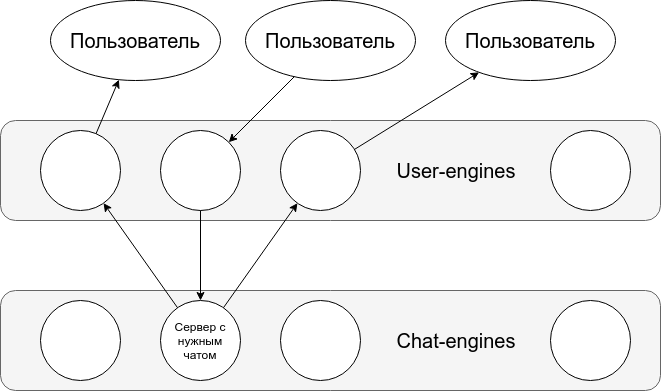
\includegraphics[width=6in]{pics/messages-structure.png}
  \caption{Отправка сообщения во <<В Контакте>>}
  \label{fig10}
\end{figure}


Когда пользователь посылает сообщение, он отправляет его в соответствующий ему user-engine, 
который, зная в какой чат послано сообщение, отправляет его в нужный chat-engine, который в свою
 очередь, рассылает данное сообщение всем участникам чата в нужные user-engine. 
Когда пользователь хочет получить сообщения, он посылает запрос соответствующему ему user-engine, 
который хранит список всех его сообщений с ссылками на нужные чаты. User-engine запрашивает нужные сообщения
 из chat-engine (либо берет их из своего кеша) и отдает пользователю.


Все эти сервисы располагаются на 500 серверах, каждый из которых имеет по 128 гигабайт оперативной
 памяти. На каждом сервере запущено восемь user-engine и восемь chat-engine (по количеству жестких 
 дисков). Каждому user-engine выделено 8 гигабайт оперативной памяти, а каждому chat-engine 4,5 
 гигабайта. Нас интересует способ хранения сообщений в chat-engine. На каждый chat-engine приходится 
 в среднем 500 миллионов сообщений суммарным размером 13 гигабайт. Из 4,5 гигабайт памяти,
 которая выделена chat-engine, он тратит примерно половину на поисковый индекс и хранение метаинформации сообщений.
 На хранение текстов сообщений остается в среднем 2,5 гигабайта.


 Таким образом, если бы удалось сжать сообщения в пять раз, то все сообщения поместились бы в память и 
 не было бы никаких проблем. Но нам не удалось достичь такой степени сжатия, поэтому сообщения подгружаются с диска
 по мере необходимости. Если же свободная память заканчивается, то сообщения чата, которые дольше всего не спрашивали,
 выгружаются из памяти.

 Из описанной архитектуры следует, что самую важную роль при выборе алгоритма сжатия играет общий размер сообщений, 
 который может быть сохранен в памяти.
 При этом следует учитывать, что данная архитектура позволяет сохранить некоторую дополнительную информацию и использовать ее
 при сжатии и разжатии данных. Можно считать, что у алгоритма есть в распоряжении примерно 2,5 гигабайта памяти, которую он 
 может использовать под дополнительную информацию (обозначим ее через $additional\ info$) и хранение сжатых сообщений ($compressed\ size$).
Обозначим суммарный размер исходных сообщений как $messages\ size$, тогда $compress\ ratio = \frac{messages\ size}{compressed\ size + additional\ info}$.
Как раз $compress\ ratio$ нам и нужно оптимизировать. Чем он больше~---тем лучше.

Также важную роль играет скорость, с которой алгоритм может сжимать и разжимает данные. 
Нельзя допустить, чтобы часто случалась ситуация, когда сообщения отдаются пользователю слишком долго. 
Это условие довольно сложно описать формально. Во-первых, чем быстрее средняя скорость сжатия/разжатия, тем лучше.
Но при этом будет плохо, если будет много случаев, когда сообщения отдаются дольше секунды. Также важно не
только время конвертации одного сообщения, но и суммарная нагрузка на процессор, которая создается за счет 
конвертации данных.

\section{Существующие алгоритмы сжатия}

На данный момент существует огромное множество алгоритмов сжатия данных. Нас интересуют только алгоритмы, которые сжимают
данные без потерь. Среди них нас интересуют те, которые ориентированы на сжатие текстовых данных. Далее будут рассмотрены некоторые из них.
Более детально можно ознакомиться с ними в \cite{handbook}.

\subsection{Run-Length encoding}
Кодирование длин серий (или RLE)~--- один из самых простых алгоритмов сжатия данных. Он работает хорошо, если в тексте много подряд идущих одинаковых символов.
Идея алгоритма заключается в том, чтобы заменить $n$ подряд идущих символов $c$ на строку $nc$. Например, строка \text{ABAAACCCCCA} будет заменена на 
\text{1A1B3A5C1A}. 

В показанном примере размер строки уменьшился с 11 символов до 10, однако очень просто привести пример на котором размер строки увеличится. 
Например, строка \text{ABC} превратится в \text{1A1B1C} и станет в два раза длиннее.

Данный метод редко используют на практике для сжатия текстовых данных, однако во многих современных алгоритмах 
сжатия текста используется LZ77, который является обобщением RLE \cite{rle-wiki}.

\subsection{LZ77}

Идея алгоритма заключается в том, чтобы ссылаться на предыдущее вхождение текста. Более формально~--- кодировщик хранит последние несколько килобайт закодированных данных,
а когда хочет закодировать очередной кусок текста, находит наибольшее вхождение текста, которое он помнит, и выписывает пару чисел, которые обозначают как давно он видел
этот текст и какой он длины.

Согласно \cite{lz77-wiki} одним из недостатков данного метода является малая эффективность при кодировании небольшого объема данных. В решаемой нами задаче средняя длина 
сообщения очень маленькая, поэтому алгоритм скорее всего не даст хороших результатов.

\subsection{PPM}

Предсказание по частичному совпадению (Prediction by Partial Matching)~--- алгоритм, который предсказывает вероятность появления очередного символа основываясь на предыдущем опыте.
Параметром модели PPM является число $n$~--- максимальный размер контекста, который анализируется. Обычно $n$ порядка нескольких символов. Для того, чтобы оценить вероятность появления 
конкретной очередной буквы рассматриваются все подстроки длины $n$, которые совпадают с последними $n$ символами. Рассматриваются все символы, которые следуют после найденных подстрок.
Если нужного символа нет, то записывается символ-исключение и рассматривается контекст размера $n - 1$ аналогичным образом. Так происходит пока не найдется подстрока, после которой идет 
нужная буква. Если такой строки найти не удалось, используется контекст степени -1, в котором есть все нужные символы.

К этому алгоритму также применяется следующая оптимизация. Если контекст длины $n$ не подошел, то точно известно, что необходимый символ точно не тот, который мог бы следовать после подстроки 
длины $n$. Поэтому вероятности этих символов при рассмотрении контекста размера $n - 1$ можно прировнять нулю.

Заметим, что данный алгоритм только предсказывает вероятность увидеть очередной символ, но не говорит как нужно кодировать данные.
Поэтому его нужно использовать вместе с алгоритмом энтропийного кодирования. Например, можно использовать алгоритм Хаффмана или арифметическое кодирование.

\subsection{Алгоритм Хаффмана}

Алгоритм Хаффмана~--- алгоритм, который был изобретен в середине прошлого века~\cite{huffman}. Идея заключается в следующем.
Пусть для каждого символа $i$ известна вероятность того, что он сейчас встретится $p_i$. Задача состоит в том,
чтобы сопоставить каждому символу битовую строку $s_i$ и минимизировать $\sum{p_i \cdot |s_i|}$. При этом необходимо,
чтобы не было двух строк таких, что одна является префиксом другой.

Оказывается, что решить эту задачу можно с помощью следующего жадного алгоритма. Рассмотрим два символа с
наименьшими вероятностями. Заменим их на один виртуальный символ, вероятность которого равна сумме вероятностей
исходных символов. Будем повторять этот процесс пока не останется один символ. После этого построим двоичное дерево 
следующим образом. Возьмем единственный символ, он будет корнем дерева. Будем повторять следующую операцию пока возможно.
Рассмотрим лист дерева, который соответствует виртуальному символу. Добавим этой вершине двух детей и скажем, что они
соответствуют символам, из которых была получена текущая виртуальная вершина.

После того как дерево построено, каждому листу в нем соответствует некоторый символ исходного алфавита. Также ему можно сопоставить 
путь из корня до него. Запишем его как битовую строку, в которой переход к левому ребенку соответствует нулю, а к правому~--- единице.
Скажем, что исходному символу соответствует полученная битовая строка.

\subsection{Арифметическое кодирование}

Недостатком алгоритма Хаффмана является то, что он не может закодировать символ нецелым числом бит. Этого недостатка лишено арифметическое кодирование.
Оно работает следующим образом. Каждому сообщению сопоставляется некоторое вещественное число, которое определяется следующим образом. Изначально берется отрезок [0, 1] и разбивается
на столько подотрезков, сколько символов алфавита. При этом размеры отрезков должны быть пропорциональны вероятности получения символа.

Перейдем к отрезку, который соответствует первому символу сообщения, и разобьем его опять в таком же соотношении (либо в другом, если вероятности встретить конкретные символы поменялись).
Перейдем в отрезок, который соответствует второму символу и так далее. После рассмотрения последнего символа выберем вещественное число из отрезка, которое записывается с помощью
наименьшего числа бит. Это и будет закодированное сообщение.

Эффективность такого сжатия строго не хуже алгоритма Хаффмана, а в большинстве случаев превосходит его. Однако, эффективная реализация данного алгоритма достаточно затруднительна. 

\subsection{Современные архиваторы}

Сейчас существует очень много различных архиваторов, но все они основаны на одних и тех же принципах, которые применяются в алгоритмах, описанных выше.
Сейчас стандартом сжатия является Deflate \cite{facebook}, который
используется в zip, gzip, zlib и других архиваторах. Сам алгоритм является смесью LZ77 и алгоритма Хаффмана.

Также интересен алгоритм zstd \cite{zstd-wiki}, который был разработан в Facebook, и сочетает в себе LZ77 и энтропийное кодирование типа Finite State Entropy.

\chapterconclusion

Существует достаточно много алгоритмов сжатия данных без потерь, некоторые из которых были рассмотрены. Поставленная задача существенно отличается от обычной задачи сжатия данных
необходимостью возможности разжимать отельные сообщения. Из-за этого большинство алгоритмов сжатия становятся неприменимы. Некоторые из них можно модифицировать таким образом,
чтобы они решали поставленную задачу. 